% Desarrollo/Analisis de resultados

%% utilice capturas de pantalla para demostrar la funcionalidad, estas capturas de pantalla deben mostrar solo la información pertinente al paso correspondiente, en esta sección es muy importante realizar un análisis de la funcionalidad del programa (utilizar diagramas de flujo, diagramas de clase, etc) y un análisis de la funcionalidad electrónica (utilizando medidas del multímetro de voltajes y/o corrientes, osciloscopio y diagramas de onda). 

\subsection{Diseño}

\subsubsection{Reescalamiento de la tensión}

Para energizar el MCU, solo se necesitan 3V ó 5V \cite{STM}, sin embargo, la fuente de energía DC será una batería de 9V. Por lo tanto, se debe disminuir la tensión haciendo uso respectivo de la técnica de división de tensión, ver ecuación \ref{ddt}. En esta ecuación, $R_1$ y $R_2$ son dos resistencia en serie, y $R_1$ comparte el nodo que la fuente de tensión de 9V.

\begin{equation}
    V_{salida}=\left ( \frac{R_{2}}{R_{1} + R_{2}} \right )\left ( V_{Bateria} \right )
    \label{ddt}
\end{equation}

Sustituyendo valores:

\begin{equation*}
    5V = \left ( \frac{R_{2}}{R_{1} + R_{2}} \right )\left ( 9V \right )
    \label{ddt}
\end{equation*}

Si $R_1 = 10k\Omega$, al despejar para $R_2$ se obtiene, $R_2 = 10k \Omega$.



\subsection{Funcionalidad del programa}

% diagrama de flujo 

%explicacion del codigo 
La programación del código para manejar el microcontrolador fue basado en los ejemplos proporcionados en el repositorio de la librería libopencm3. Con el programa realizado en el lenguaje C, se maneja el uso del giroscopio, la comunicación USART, ADC (convertidor analógico a digital) para lectura de voltaje, y el manejo de entradas/salidas digitales (GPIOs) para el control de LEDs y botones. Basándose en bibliotecas y dependencias, se utilizan archivos cabeceras proporcionados por los ejemplos de la librería.\\

Entre las funciones utilizadas, se encuentras las siguientes:
\begin{itemize}
    \item \textbf{spi\_setup}: configura la comunicación SPI necesaria para interactuar con el giroscopio, entre eso se encuentra la selección del chip (CS), configuración de los pines SPI y parámetros de la comunicación SPI. 
    \item \textbf{usart\_setup}: para la configuración de la comunicación USART que va a permitir la transmisión de datos a través del puerto serial.
    \item \textbf{gpio\_setup}: se configuran los pines GPIO a utilizar del LED. 
    \item \textbf{button\_setup}: para la inicialización del botón de la placa. 
    \item \textbf{clock\_setup\_G}: se configura el sistema de relojes del MCU, y se habilita el clock para los periféricos utilizados.
    \item \textbf{adc\_setup}: se inicializa el ADC para leer valores analógicos, y es utilizado para monitorear el voltaje de la batería.
    \item \textbf{my\_usart\_print\_int}: envía un número entero por medio del USART, y se formatea el número como cadena.
\end{itemize}

A través del main, se inicializa el programa y se configuran los periféricos. Luego se entra en un loop infinito while donde se van a leer los datos del giroscopio mediante SPI, y se presentan las lecturas de los ejes X, Y, Z en el display LCD incorporado en el kit del stm32. Con el adc, se programa para medir el valor del voltaje de la batería, donde también se muestra en la pantalla y se emplea el LED de la placa para señalar el estado de carga. Otra función del código consiste en la habilitación de la transmisión USART usando el botón del MCU, donde se indica su estado (activado o desactivado) en el display y transmite la información de los ejes por USART al estar activo. En la pantalla lcd del stm32 se logra imprimir los datos gracias al archivo header gfx.h, con el cual se puede definir el color, tamaño y posición del texto a mostrar. Se destaca que se agrega un pequeño delay en la toma de datos del giroscopio para poder tener una mejor y correcta visualización de los datos, así como un delay en el botón para evitar el efecto rebote que puede provocar lecturas poco precisas.  \\

Adicional a este programa, se realiza un script en python donde al correrlo se obtiene la lectura de datos de los ejes X Y y Z, así como el estado de la batería, todo esto en caso de que se encuentre habilitado la comunicación serial. Con el script, se logra la lectura de datos desde un puerto serie y la publicación de estos datos a un servidor MQTT en el puerto 1883. Para publicar los mensajes en la consola se utiliza el tópico MQTT v1/devices/me/telemetry a una velocidad de baudios de 115200. Se definen los manejadores de eventos para conectarse (la función on\_connect) y desconectarse (con la función on\_disconnect) del servidor MQTT, para así imprimir los mensajes de estado sobre la conexión. Se tiene un loop infinito donde si hay datos disponibles en el puerto serie, los lee, decodifica a texto (UTF-8), y los procesa. Para analizar los datos leídos del puerto serie, se construye un payload JSON con los valores de los ejes X, Y, Z y lo publica en el topic MQTT configurado. 


\subsection{Funcionalidad electrónica}

\subsubsection{Divisor de tensión}

Se emplea una batería de 9 V para utilizar como fuente de alimentación del microcontrolador, sin embargo este dispositivo se enciende con tensión de alimentación de 3.3V y soporta hasta 5 V. Por lo que se realiza una división de tensión con resistencias para reducir la tensión de 9 V a un valor suficiente para prender el microcontrolador pero que no supere el límite de tensión admitida para evitar daños en el equipo. Se utilizan dos resistencias en serie de $10k\Omega$

\begin{figure}[H]
        \centering
        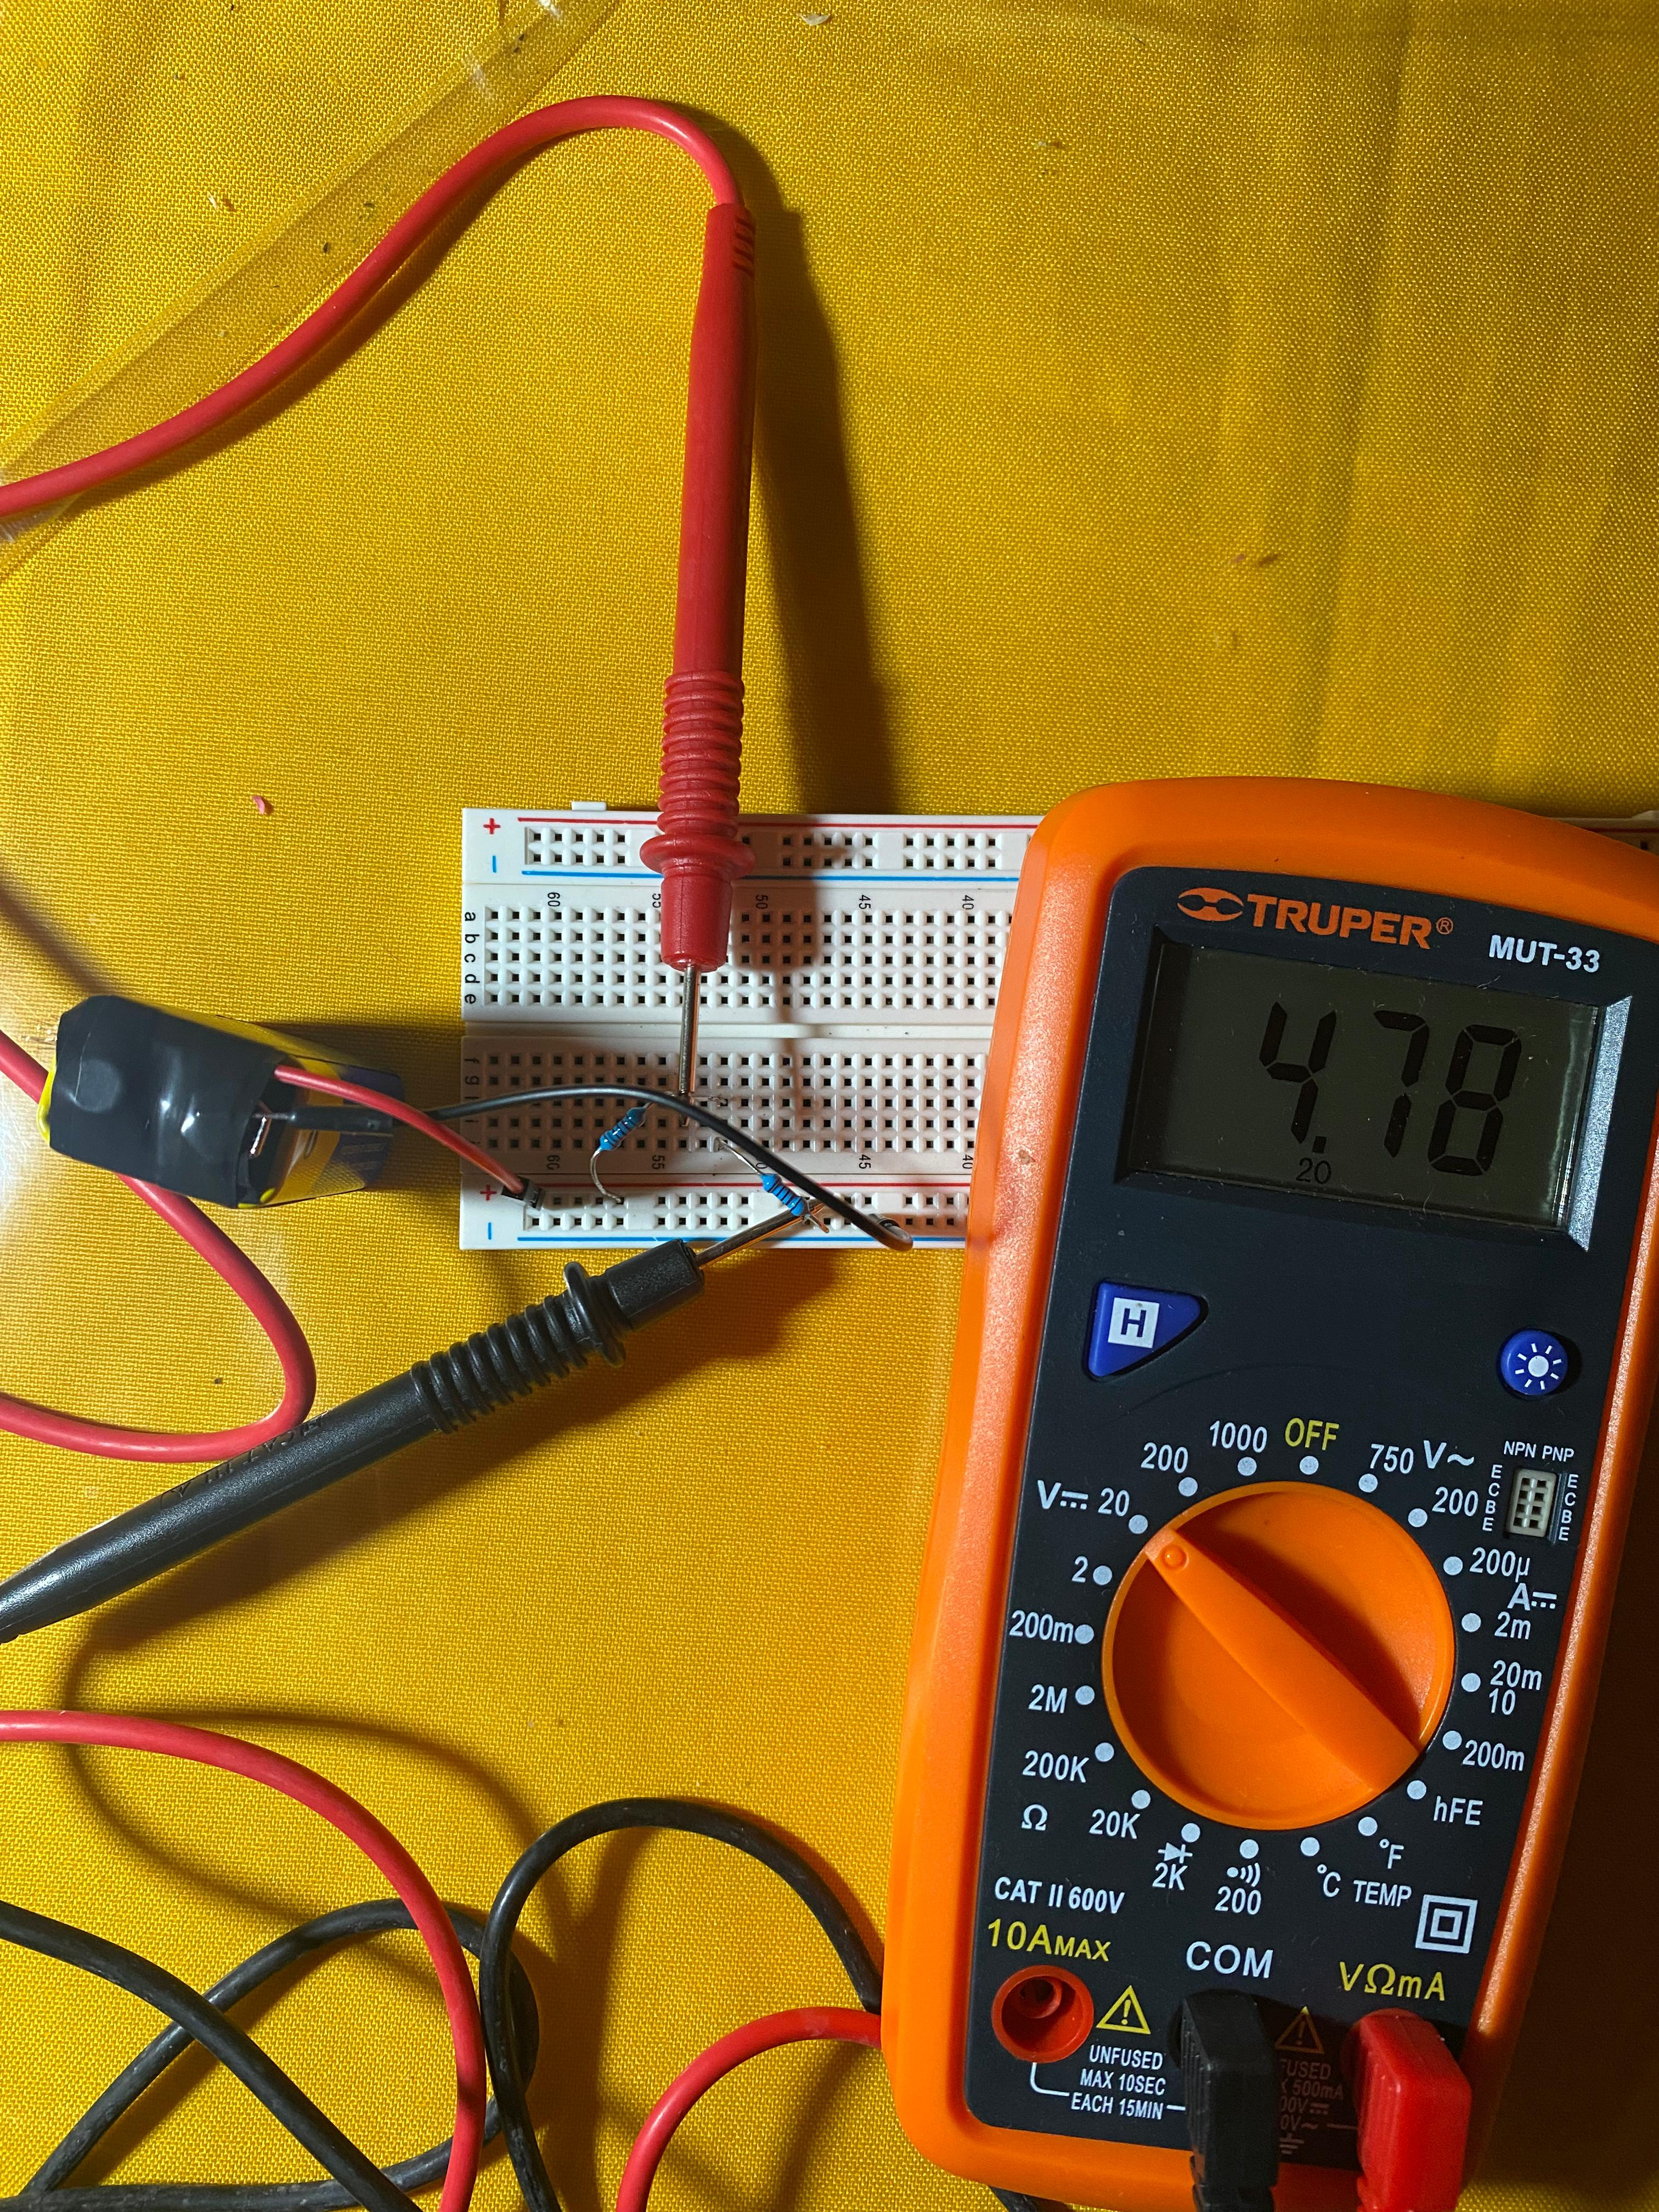
\includegraphics[width=0.5\linewidth]{fotos/voltaje.jpeg}
        \caption{Divisor de tensión para que al pin le lleguen menos de 5V a partir de una batería de 9V}
        \label{voltaje}
    \end{figure}
    
\subsubsection{Microcontrolador STM32F429}

En la figura \ref{completo} se aprecia el circuito final completo. Notar que la batería indica 9V porque está recién instalado el circuito y por ende, la carga de la batería está en lo máximo. 

\begin{figure}[H]
        \centering
        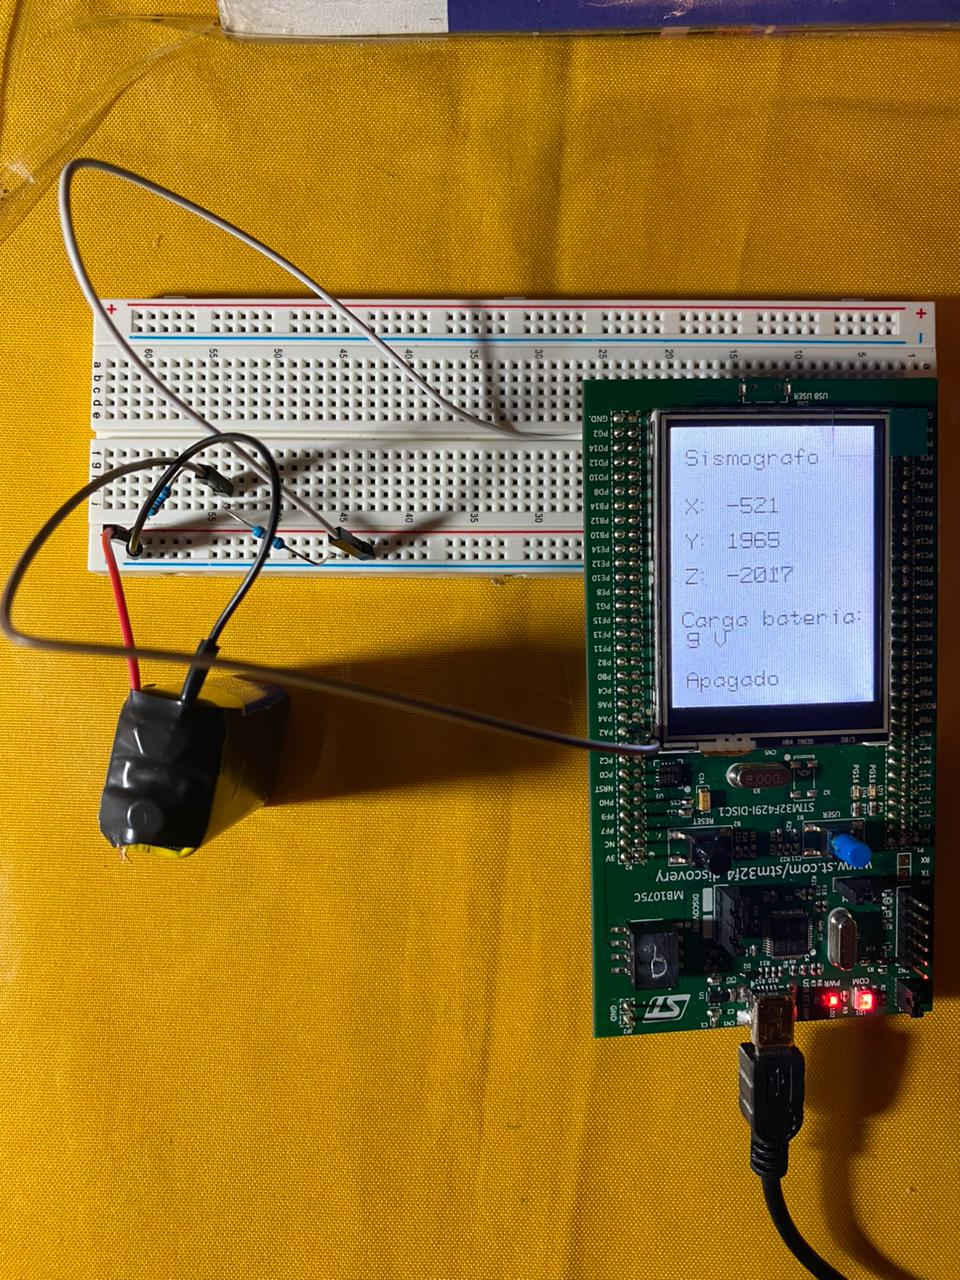
\includegraphics[width=0.7\linewidth]{fotos/completo.jpeg}
        \caption{Circuito completo con resistencias, batería y MCU.}
        \label{completo}
    \end{figure}

\begin{figure}[H]
        \centering
        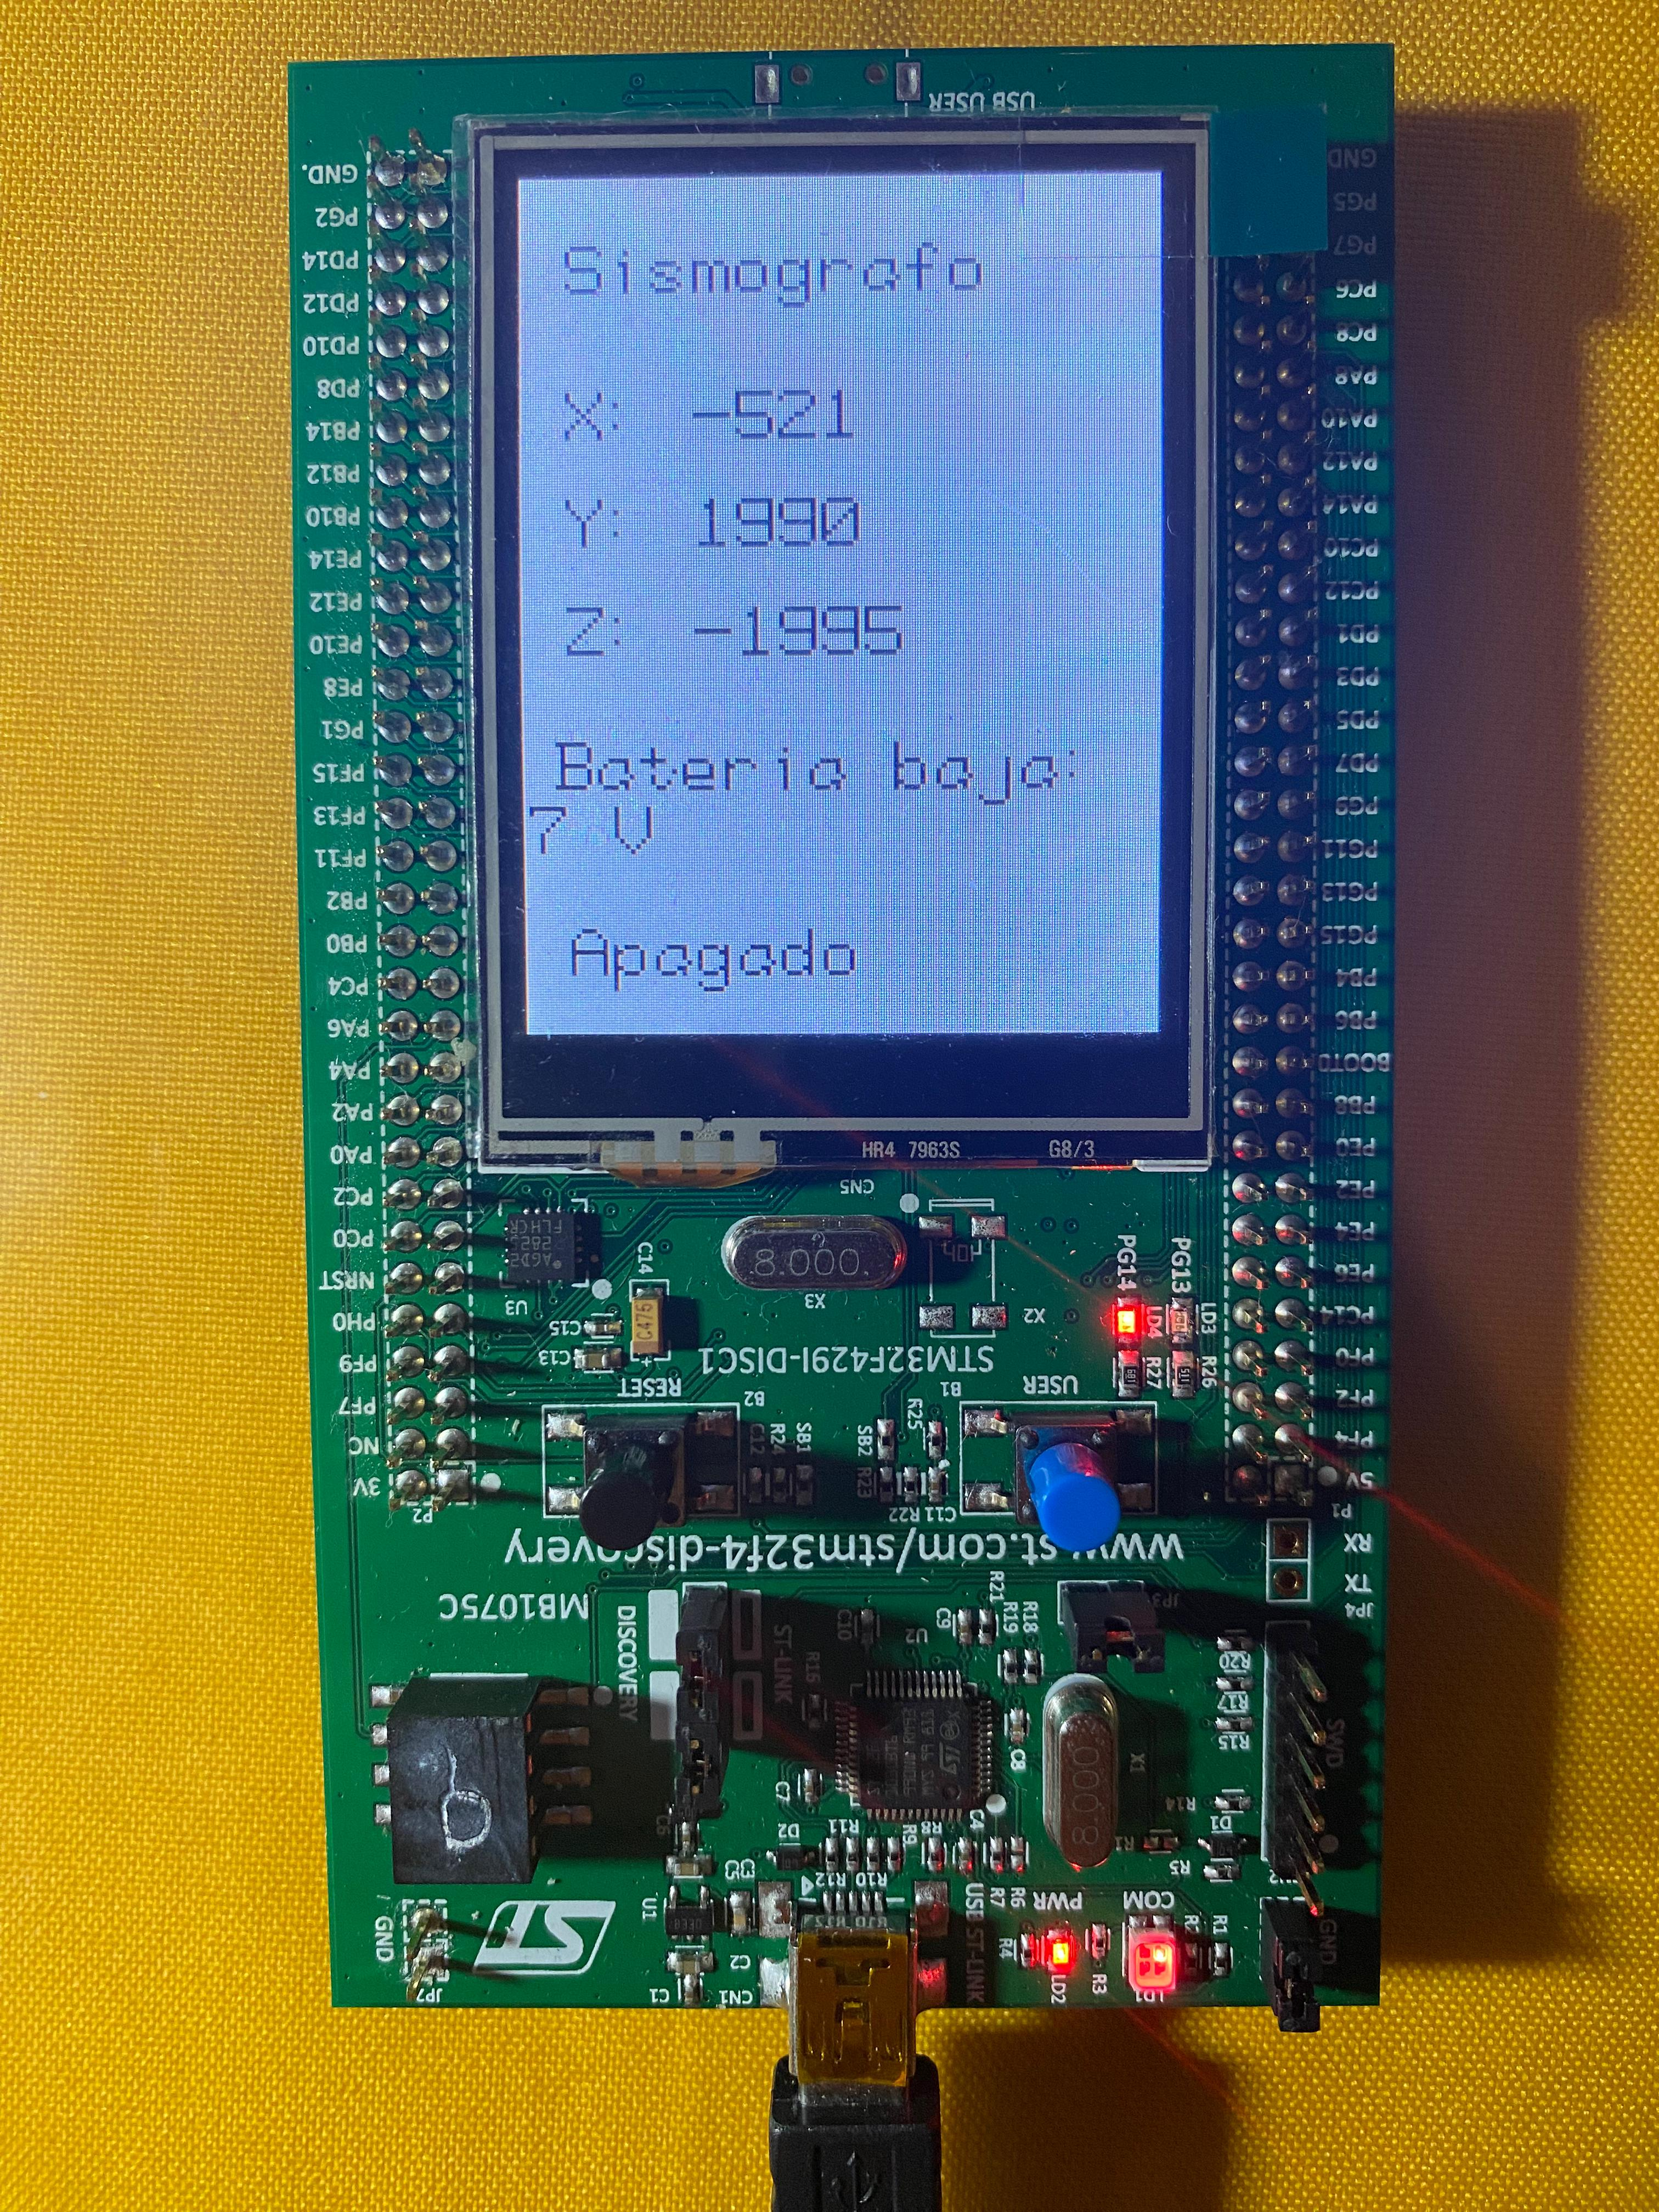
\includegraphics[width=0.5\linewidth]{fotos/bate_baja_apagada.jpeg}
        \caption{MCU muestra valores de los ejes, el nivel bajo de la batería y la transmisión de datos hacia el dashboard apagada.}
        \label{bate_baja_apagada}
    \end{figure}
    
\begin{figure}[H]
        \centering
        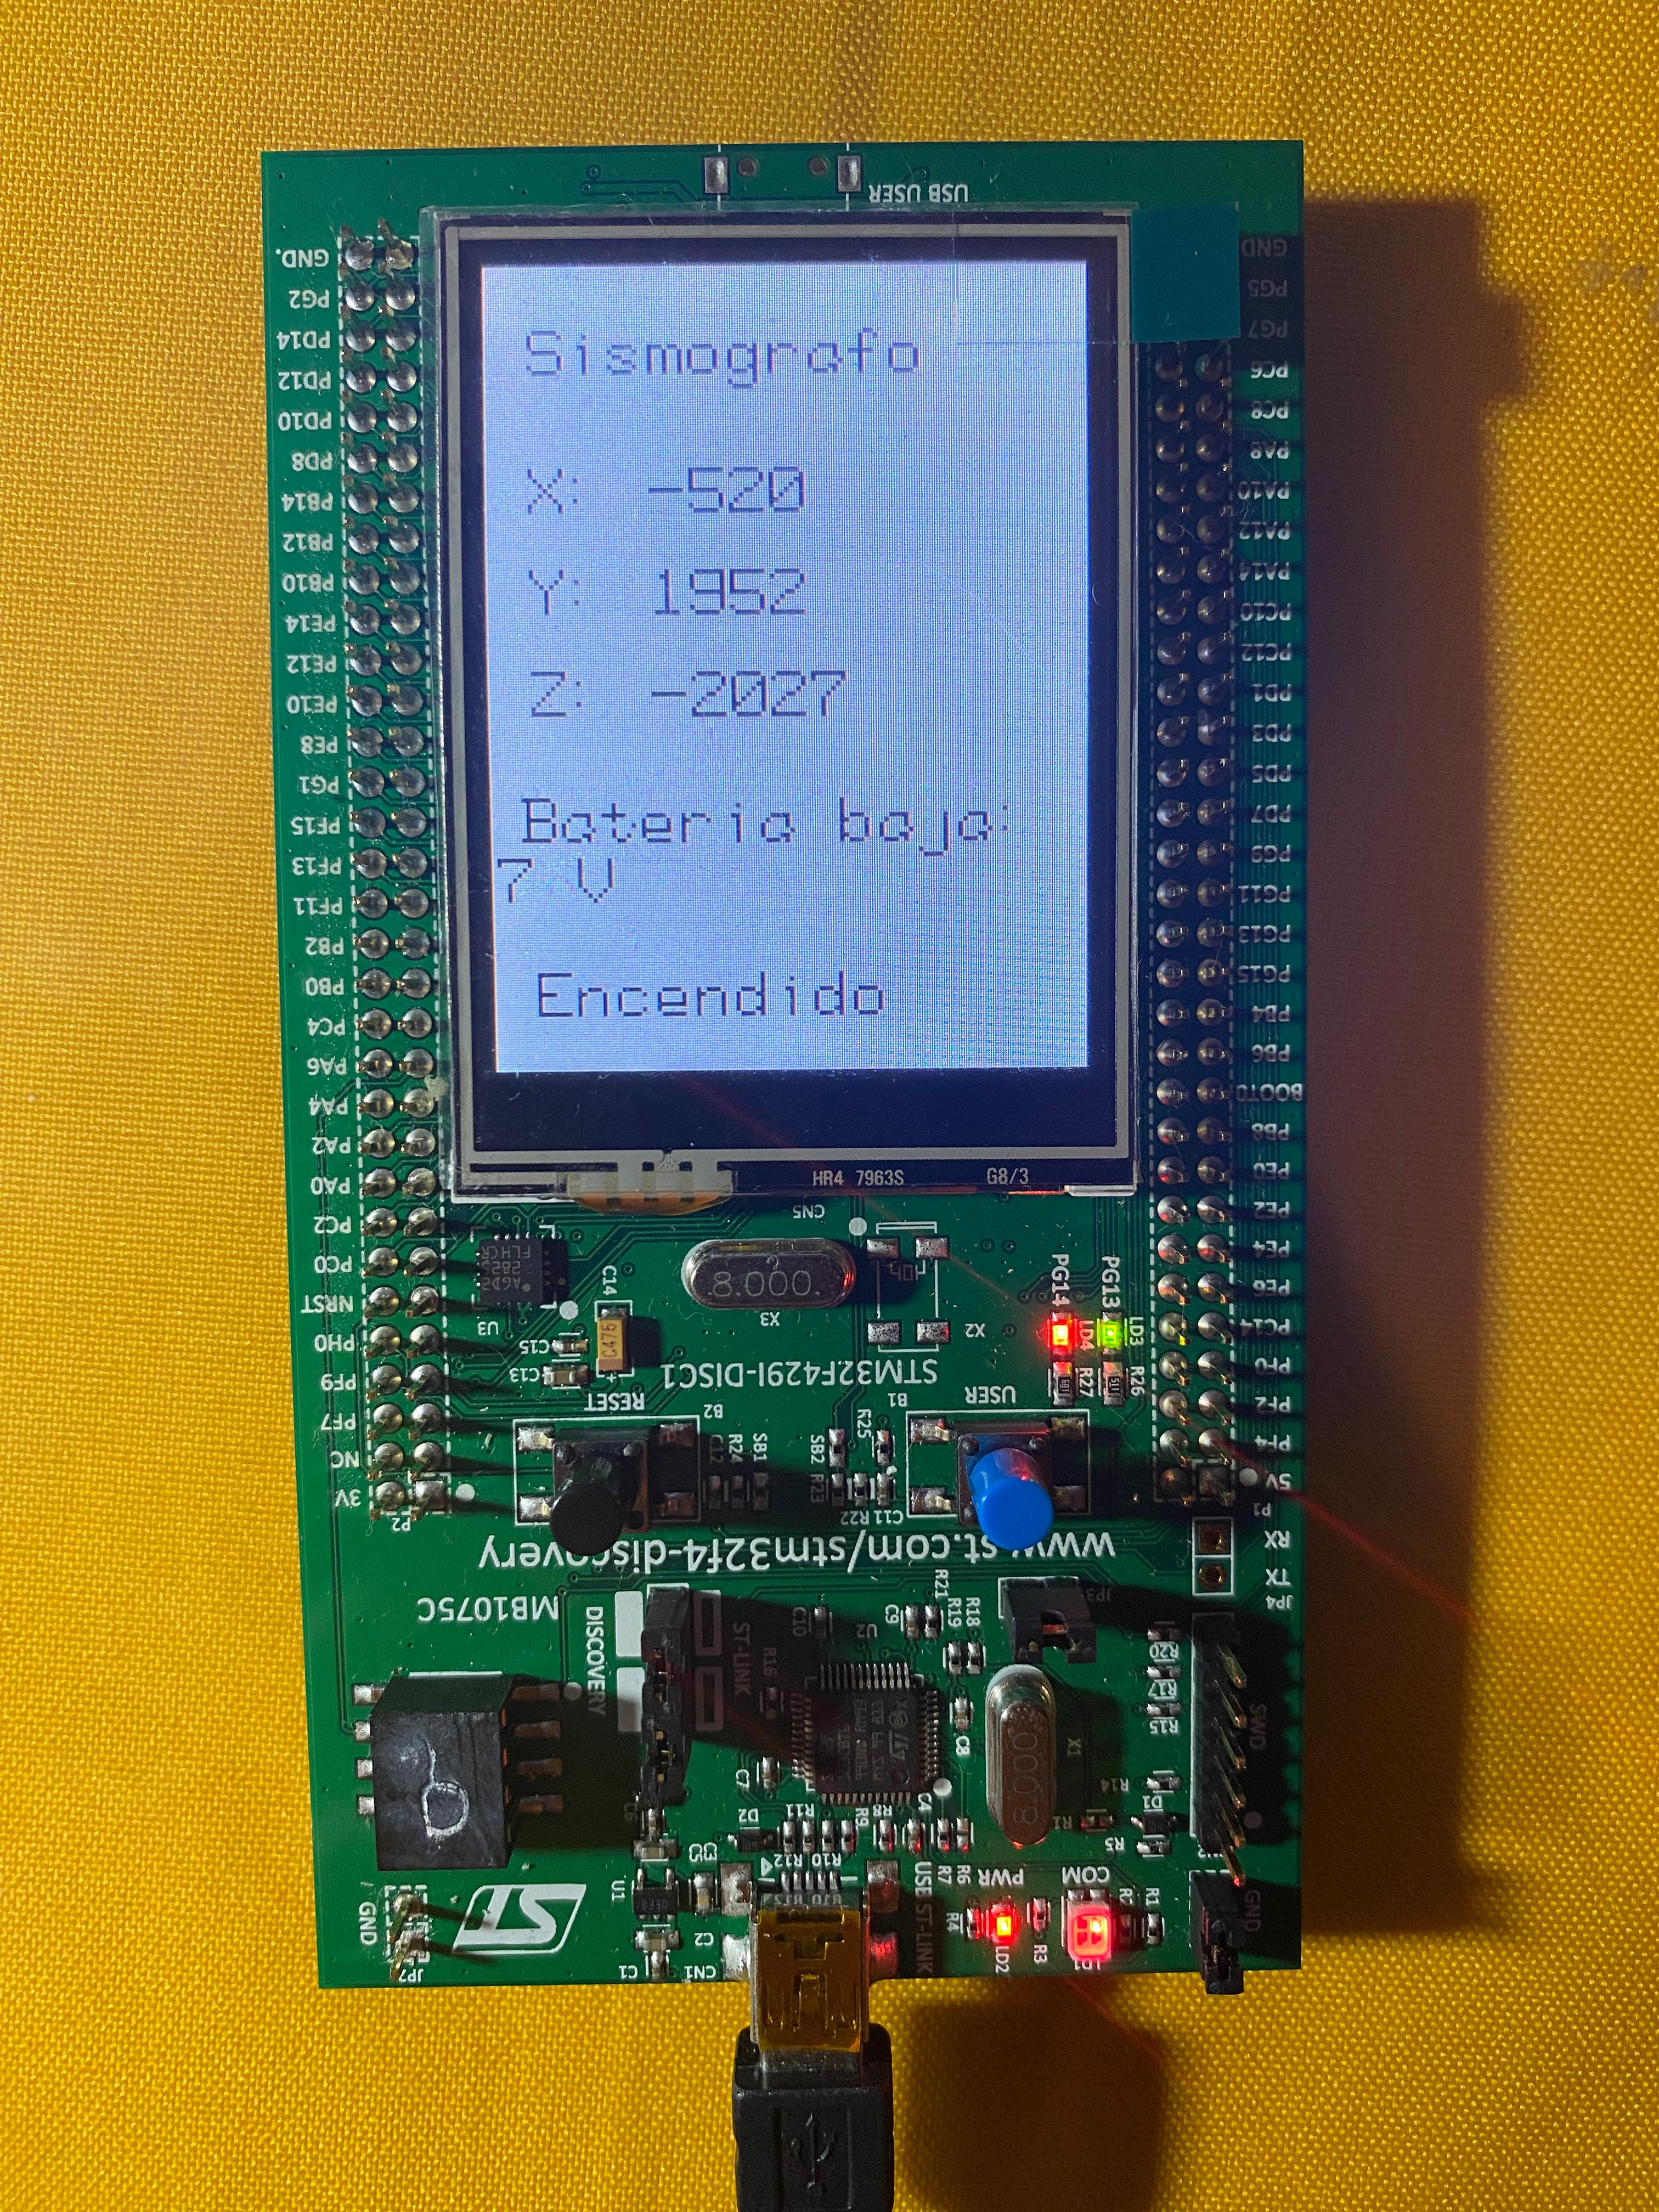
\includegraphics[width=0.5\linewidth]{fotos/bate_baja_encendido.jpeg}
        \caption{MCU muestra valores de los ejes, el nivel bajo de la batería y la transmisión de datos hacia el dashboard encendida.}
        \label{bate_baja_encendido}
    \end{figure}

\subsubsection{Dashboard en ThingsBoard}

Mediante la plataforma IoT en línea de ThingsBoard se configura para la gestión de dispositivos recopilación de datos, procesamiento y visualización para su IoT (Internet of Things). En el script de python realizado, se ingresa el usuario y contraseña así como el número de dispositivo para lograr su conexión con el dashboard. En los siguientes figuras, se observan los widgets empleados para la visualización de los datos obtenidos, donde se utiliza un widget que funciona como una gráfica de línea del tiempo con la cual se registra el promedio de los valores de los ejes. Luego se emplea un widget con el que se puede ver el nivel de tensión de la batería actualmente.

\begin{figure}[H]
        \centering
        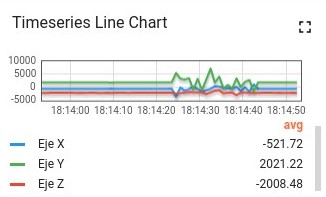
\includegraphics[width=0.5\linewidth]{fotos/temblor.jpg}
        \caption{Transmisión de datos encendida y con movimiento en dashboard.}
        \label{temblor}
    \end{figure}


\begin{figure}[H]
        \centering
        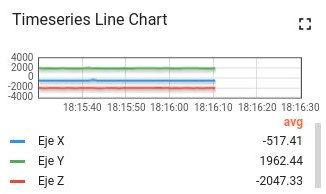
\includegraphics[width=0.5\linewidth]{fotos/apagado.jpg}
        \caption{Transmisión de datos apagada en dashboard.}
        \label{apagado}
    \end{figure}

En la figura \ref{apagado2} se observa el widget para el nivel de batería, al momento de la toma está la batería al máximo pero conforme la batería se vaya descargando este widget indicará una voltaje menor. 

    \begin{figure}[H]
        \centering
        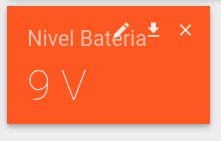
\includegraphics[width=0.4\linewidth]{fotos/nueve.jpg}
        \caption{Transmisión de datos encendida para el nivel de batería.}
        \label{apagado2}
    \end{figure}


Gracias al widget utilizado en el dashboard, llamado Timeseries Line Chart, se puede hacer un emulador de sismógrafo donde si no hay movimiento como se observa en la figura \ref{apagado}, entonces las líneas se mantienen constantes en un valor promedio. Cuando hay movimiento, es decir un temblor, las líneas de la gráfoca van a aumentar y moverse hasta llegar al punto de estabilidad tal como sucedería con un sismógrafo real que detecta un movimiento sísmico. 